\documentclass[11pt]{article}

\usepackage{ifpdf}
\usepackage{booktabs}
\usepackage{array}
\usepackage{paralist}
\usepackage{subfigure}
\usepackage[pdftex]{graphicx}
\usepackage{epstopdf}
\usepackage[cmex10]{amsmath}
\interdisplaylinepenalty=2500
\usepackage{geometry}
\geometry{letterpaper}
\usepackage{fancyhdr}
\pagestyle{fancy}
\renewcommand{\headrulewidth}{0pt}
\lhead{}\chead{}\rhead{}
\lfoot{}\cfoot{\thepage}\rfoot{}

\usepackage{amsfonts}
\usepackage{amstext}
\usepackage{booktabs}
\usepackage{threeparttable}
\usepackage{longtable}
\usepackage{listings}
\usepackage[font=normalsize]{caption}
\usepackage{textcomp}
\usepackage[usenames]{color}
\usepackage{soul}
\usepackage{fancyvrb}
\usepackage{relsize}
\usepackage[noadjust]{cite}
\usepackage{xr-hyper}
\usepackage[usenames,dvipsnames,svgnames,table]{xcolor}
\usepackage[colorlinks=true,linkcolor=black,urlcolor=blue,hyperfootnotes=false,backref=section,citecolor=LimeGreen]{hyperref}
\usepackage{upquote}
\usepackage[title,titletoc]{appendix}

\usepackage[nottoc,notlof,notlot]{tocbibind}
%\renewcommand{\FancyVerbFormatLine}[1]{\makebox[2mm][l]{}#1}
%\DefineVerbatimEnvironment%
%  {Code}{Verbatim}
%  {fontsize=\relsize{-1.5},
%  samepage=true,
%  frame=single}

\renewcommand{\FancyVerbFormatLine}[1]{\makebox[2mm][l]{}#1}
\DefineVerbatimEnvironment%
  {Notice}{Verbatim}
  {fontsize=\relsize{-1.5},
  samepage=true,
  xleftmargin=15mm,
  framesep=5mm,
  frame=single}

\newcommand{\covemda}{CoVEMDA}
\newcommand{\covemdagithuburl}{https://github.com/tamu-engineering-research/COVID-EMDA}
\newcommand{\matlab}{\textsc{MATLAB}}

\definecolor{BackgroundColor}{HTML}{e7f2fa}
\definecolor{SepColor}{HTML}{6ab0de}
\definecolor{DarkGreen}{rgb}{0.0,0.4,0.0}

\lstnewenvironment{Code}
    {\lstset{
        language=matlab,
        frame=shadowbox, 
        frameshape={RYRYNYYYY}{yny}{yny}{RYRYNYYYY},
        basicstyle=\ttfamily,
        commentstyle=\color{DarkGreen},
        stringstyle=\color{purple},
        keywordstyle=\bfseries\color{blue},
        backgroundcolor=\color{BackgroundColor}%
        %rulesepcolor=\color{SepColor}%
        }}
    {}

        
\def\sectionautorefname{Chapter}
\def\subsectionautorefname{Section}
\def\subsubsectionautorefname{Section}
\newcommand{\secref}[1]{\autoref{#1} \nameref{#1}}

\numberwithin{equation}{section}
\numberwithin{table}{section}
\renewcommand{\thetable}{\thesection\mbox{-}\arabic{table}}
\numberwithin{figure}{section}
\renewcommand{\thefigure}{\thesection\mbox{-}\arabic{figure}}



%%% title setting
\title{User's Manual for CoVEMDA Toolbox}
\author{}
\date{\today}
%\date{December 14, 2011\thanks{Second revision. First revision wyas December 13, 2011}} % comment this line to display the current date



%%% BEGIN DOCUMENT
\begin{document}
\maketitle
\thispagestyle{empty}
\newpage
\tableofcontents
\thispagestyle{empty}


%-------------------------------
\newpage
\setcounter{page}{1}
\section*{Website}
\addcontentsline{toc}{section}{Website}

\url{https://github.com/tamu-engineering-research/COVID-EMDA}

\begin{center}
	\noindent
\includegraphics[width=0.5\textwidth]{figures/covid_emda_logo.JPG}
\end{center}



%-------------------------------
\newpage
\section{Introduction} \label{sec:intro}

\subsection{Background}

\subsection{Features}
\begin{itemize}
    \item[$\bullet$] Overall, this data hub contains the \textbf{coronavirus case \& deaths}, \textbf{weather}, \textbf{generation mix}, \textbf{load} and \textbf{price} data for \textbf{all the existing U.S. electricity marketplaces}\footnote{Which refers to CAISO, MISO, ISO-NE, NYISO, PJM, SPP, ERCOT, see more in Section ~\ref{sec:datahub}} and some typical cities\footnote{Which refers to Los Angeles, Boston, New York City, Philadelphia, Chicago, Kansas City, Houston} in these markets. We also integrate other additional resources, including the \textbf{mobile device location}, \textbf{night-time lighting images}, \textbf{load forecasting}, \textbf{congestion price}, \textbf{forced outage} and \textbf{renewable curtailment} data. 
    \item[$\bullet$] This data hub is updated every day after careful \textbf{quality control}. All data are carefully verified and coordinated to match the geological scale. All data are recorded and tidied in a consistent, compact and ready-to-use data format that makes it easy for cross-market analysis.
    \item[$\bullet$] A supplementary toolbox on the basis of some useful parsers with other resources has been designed for further analysis as well as other user-defined extensions. The toolbox, implemented both in Python and MATLAB language, can guarantee you the easy access to \textbf{data visualization}, \textbf{baseline-estimation} and \textbf{regression analysis}.
\end{itemize}

\textbf{Note}: Historical data dating back to 2017 are included as time-series benchmarks.

\subsection{Support Team}
This project is a collaboration of our group members under the supervision of Prof. Le Xie at Texas A\&M University. The support team keeps processing, correcting and updating the data every day. The team will also conduct further research analysis and share the latest progress in this repository.

\begin{figure}[!ht]
    \centering
    
\includegraphics[width=.7\textwidth]{figures/contributor-0725.png}
    \caption{Support Team}
\end{figure}

Please also check our \href{https://gridx.engr.tamu.edu/?page_id=30}{Group Website} for the detailed biography of each group member.

\subsection{Suggested Citation}
Publications originated from the employment of data files in COVID-EMDA+, or the supplementary toolbox, are requested to cite the following paper explicitly and properly: 

\begin{quotation}\footnotesize
G. Ruan, D. Wu, X. Zheng, H. Zhong, C. Kang, M. A. Dahleh, S. Sivaranjani, and L. Xie, ``A Cross-Domain Approach to Analyzing the Short-Run Impact of COVID-19 on the U.S. Electricity Sector,'' Joule, 2020. (Accepted)
\end{quotation}

This paper conducts a comprehensive introduction of this data hub and further analysis results for electricity demand across the U.S. Its full text is available at: \href{https://arxiv.org/abs/2005.06631}{arXiv} and \href{http://www.enerarxiv.org/page/thesis.html?id=1840}{EnerarXiv}.

Other research studies of our group are recommended to be cited as:

\begin{quotation}\footnotesize
G. Ruan, J. Wu, H. Zhong, Q. Xia, and L. Xie, ``Quantitative Assessment of U.S. Bulk Power Systems and Market Operations during the COVID-19 Pandemic,'' 2020. (Submitted to Applied Energy)
\end{quotation}

This paper substantiates the pandemic's impacts from the perspectives of power system security, electric power generation, electric power demand and electricity prices. Its full text is available at: \href{http://www.enerarxiv.org/page/thesis.html?id=2196}{EnerarXiv}.

\begin{quotation}\footnotesize
H. Zhong, Z. Tan, Y. He, L. Xie, and C. Kang, ``Implications of COVID-19 for the Electricity Industry: A Comprehensive Review'', CSEE Journal of Power and Energy Systems, 2020.
\end{quotation}

This paper provides a review of the global impacts that COVID-19 has caused on the electricity sector. Its full text is available at: \href{https://ieeexplore.ieee.org/abstract/document/9160443}{JPES}.

\subsection{License}
The code of \covemda~is licensed under the \textbf{MIT License}, the full text of which can be found at the top level of distribution or \url{https://github.com/tamu-engineering-research/COVID-EMDA/blob/master/LICENSE} and reads as follows.
\begin{Notice}
Copyright (c) 2020 Guangchun Ruan

Permission is hereby granted, free of charge, to any person obtaining a copy
of this software and associated documentation files (the "Software"), to deal
in the Software without restriction, including without limitation the rights
to use, copy, modify, merge, publish, distribute, sublicense, and/or sell
copies of the Software, and to permit persons to whom the Software is
furnished to do so, subject to the following conditions:

The above copyright notice and this permission notice shall be included in all
copies or substantial portions of the Software.

THE SOFTWARE IS PROVIDED "AS IS", WITHOUT WARRANTY OF ANY KIND, EXPRESS OR
IMPLIED, INCLUDING BUT NOT LIMITED TO THE WARRANTIES OF MERCHANTABILITY,
FITNESS FOR A PARTICULAR PURPOSE AND NONINFRINGEMENT. IN NO EVENT SHALL THE
AUTHORS OR COPYRIGHT HOLDERS BE LIABLE FOR ANY CLAIM, DAMAGES OR OTHER
LIABILITY, WHETHER IN AN ACTION OF CONTRACT, TORT OR OTHERWISE, ARISING FROM,
OUT OF OR IN CONNECTION WITH THE SOFTWARE OR THE USE OR OTHER DEALINGS IN THE
SOFTWARE.
\end{Notice}






%-------------------------------
\newpage
\section{Getting Started} \label{sec:start}

\subsection{System Requirements}
To use \covemda~Toolbox you will need: MATLAB\textsuperscript{\tiny \textregistered} version 9.8 (R2020a). 

\small\emph{
\begin{enumerate}[NOTE 1]
    \item Despite the fact that \textbf{GNU Octave} can also tackle \textsf{.m} files, several functions like \textsf{isdatetime}  have not been implemented in \textbf{GNU Octave} (even the latest 6.1.0).
    \item For those who want long-term data support, \textbf{Git}\footnote{``Git is a free and open-source distributed version control system.'' It can guarantee you the easy access to the latest released data in multiple platforms. Git is available on its \href{https://git-scm.com/}{official website}, where both command-line version and gui version are provided.}/\textbf{GitHub Desktop}\footnote{``GitHub Desktop extends and simplifies your Git and GitHub workflow using a visual interface.'' Only systems of macOS and Windows are supported. The software is accessible at \url{https://desktop.github.com/}, while docs are available at \url{https://docs.github.com/en/desktop}} are needed for your latter convenience.
\end{enumerate}    
}

As for the hardware requirements, please refer to the System Requirements of MATLAB according to the specific version\footnote{\url{https://www.mathworks.com/support/requirements/previous-releases.html}}.

\subsection{Getting Data and Toolbox}
Our distribution containing COVID-EMDA data hub and toolbox can be obtained from the GitHub repository. You can either download the whole package of a specific distribution, or subscribe the daily-updated data via cloning the repository to your local folder.

\subsubsection{Download Specific Distribution}
    To get a specific distribution, please download the compressed zip-file of GitHub repository, as seen in Figure~\ref{fig:githubwebsite}.
    \begin{itemize}
        \item Go to \href{\covemdagithuburl}{\covemda~GitHub repository} by browser.
        \item Click the green \textbf{Code} button.
        \item Click the \textbf{Download ZIP} button.
        \item Uncompress the zip file to certain directory.
        \begin{figure}[htbp]
            \centering
            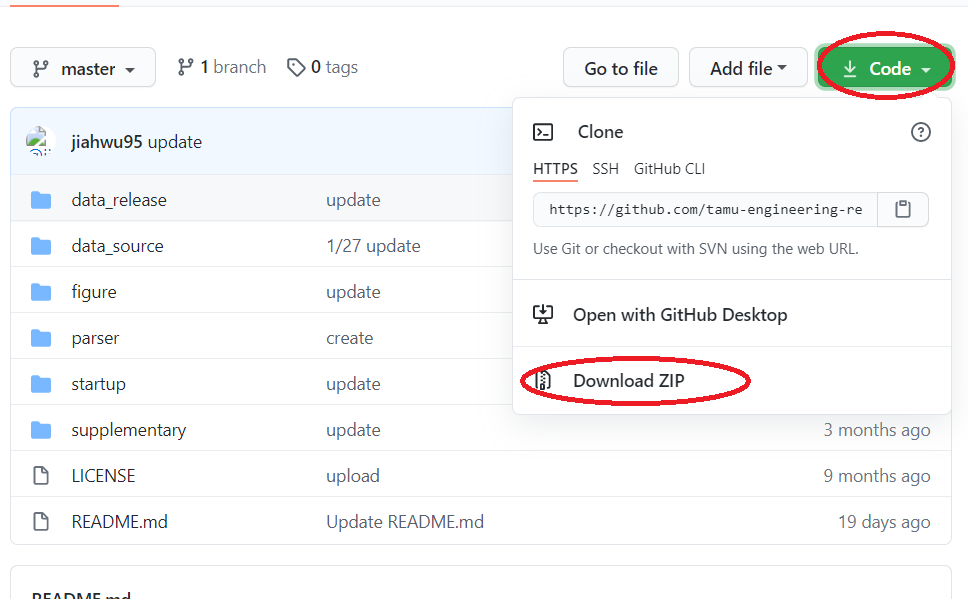
\includegraphics[width=.7\textwidth]{figures/github_website_step_1.png}
            \caption{Download from GitHub Website}
            \label{fig:githubwebsite}
        \end{figure}
    \end{itemize}
\textbf{Note}: Use this option to obtain updated data or new features of toolbox, if you are unfamiliar with or have no access to \textbf{Git}/\textbf{GitHub Desktop}.\footnote{But it would not be a bad idea to give \textbf{Git}/\textbf{GitHub Desktop} a try.}


\subsubsection{Clone GitHub Repository}
    \textbf{Git} (Either command-line or gui version is OK.) or \textbf{GitHub Desktop} is required to clone GitHub repository.
    \begin{itemize}
        \item \textbf{Git} required. Open the \textbf{Git Bash} at certain file folder (the one you want the software to be placed in) and type the following command:

\verb!git clone https://github.com/tamu-engineering-research/COVID-EMDA.git!

        \item Or if you are unfamiliar with \textbf{Git Bash}, open \textbf{Git GUI} and 
        \begin{enumerate}
            \item Click the \textbf{Clone Existing Repository} button.
            
            \begin{figure}[htbp]
                \centering
                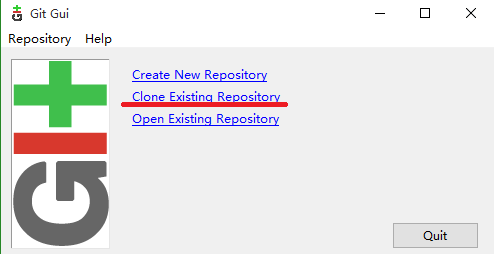
\includegraphics[width=.7\textwidth]{figures/git_gui_step_1.png}
                \caption{Git GUI: Click \textbf{Clone Existing Repository}}
            \end{figure}

            \item Type in ``https://github.com/tamu-engineering-research/COVID-EMDA.git'' in Source Location.
            \item Choose the local folder of your project, e.g., \verb!My Project! under disk G.
            
            \begin{figure}[htbp]
                \centering
                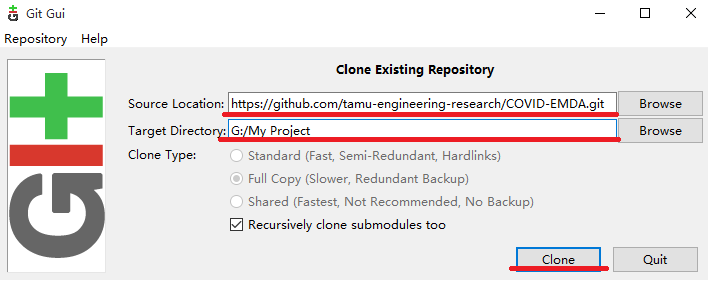
\includegraphics[width=.7\textwidth]{figures/git_gui_step_2.png}
                \caption{Git GUI: Filling two blanks}
            \end{figure}

            \item Click the \textbf{Clone} button and wait.
    
        \end{enumerate}

        \item \textbf{Github Desktop} required. 
        \begin{enumerate}
            \item Click \textbf{Clone repository...} under the \textbf{File} menu bar. 
            \begin{figure}[htbp]
                \centering
                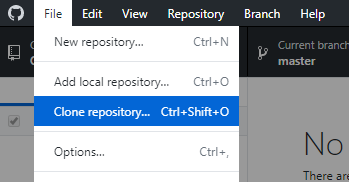
\includegraphics[width=.7\textwidth]{figures/github_desktop_step_1.png}
                \caption{GitHub Desktop: \textbf{Clone repository} in the menu bar}
            \end{figure}
            \item Choose \textbf{URL} and input \verb!username/repository! as follows: 
            
            \verb!tamu-engineering-research/COVID-EMDA!

            \begin{figure}[htbp]
                \centering
                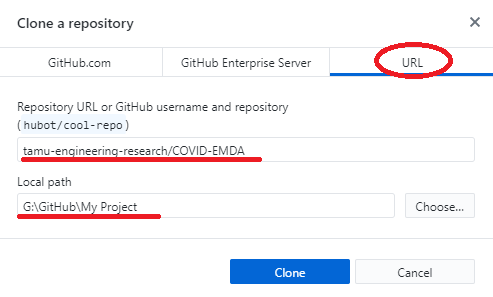
\includegraphics[width=.7\textwidth]{figures/github_desktop_step_2.png}
                \caption{GitHub Desktop: Choose source and local path}
            \end{figure}

            \item Choose your local repository path and click \textbf{Clone}.
        \end{enumerate}
    \end{itemize} 

\clearpage
\subsection{Running an Example}





%----------------------------------------
\newpage
\section{Data Hub} \label{sec:datahub}

\subsection{Data Category}

\subsection{Data Structure}

\subsection{Field Description}

\subsection{Quality Control}








%--------------------------------------------
\newpage
\section{Visualization} \label{sec:visual}

\subsection{Generation Mix}

In this section, we provide two typical tools to display the generation data of U.S. electricity markets. After the COVID-19 outbreak, the total generation as well as generation share of each market in U.S. varied. In order to analyse this change, we may observe the generation data in scale of time or of generation fuels. This may offer a new approach for researchers to find out the structure change of U.S. power grid brought by COVID-19.

In \covemda{}, two typical tools regarding different scales are provided for generation analysis: \verb!plot_generation_mix! and \verb!plot_renewable_share!. Both of them obtain relevant data from file \verb!<market_name>_rto_genmix.csv! in the data hub.


\subsubsection{plot generation mix}

This function plots the generation mix of a market within specified date range. Like \verb!area!, it returns the area objects of the curve for further modification.

\begin{Code}
  ar = plot_generation_mix(market,Name,Value)
\end{Code}

This function is based on \matlab{} function \verb!area!.

By default, the function plots the generation mix of the specified market from 2017-01-01 to 2020-07-15, with month resampling.

\begin{Code}
  >> plot_generation_mix('spp');
\end{Code}

\begin{figure}
  \centering
  \noindent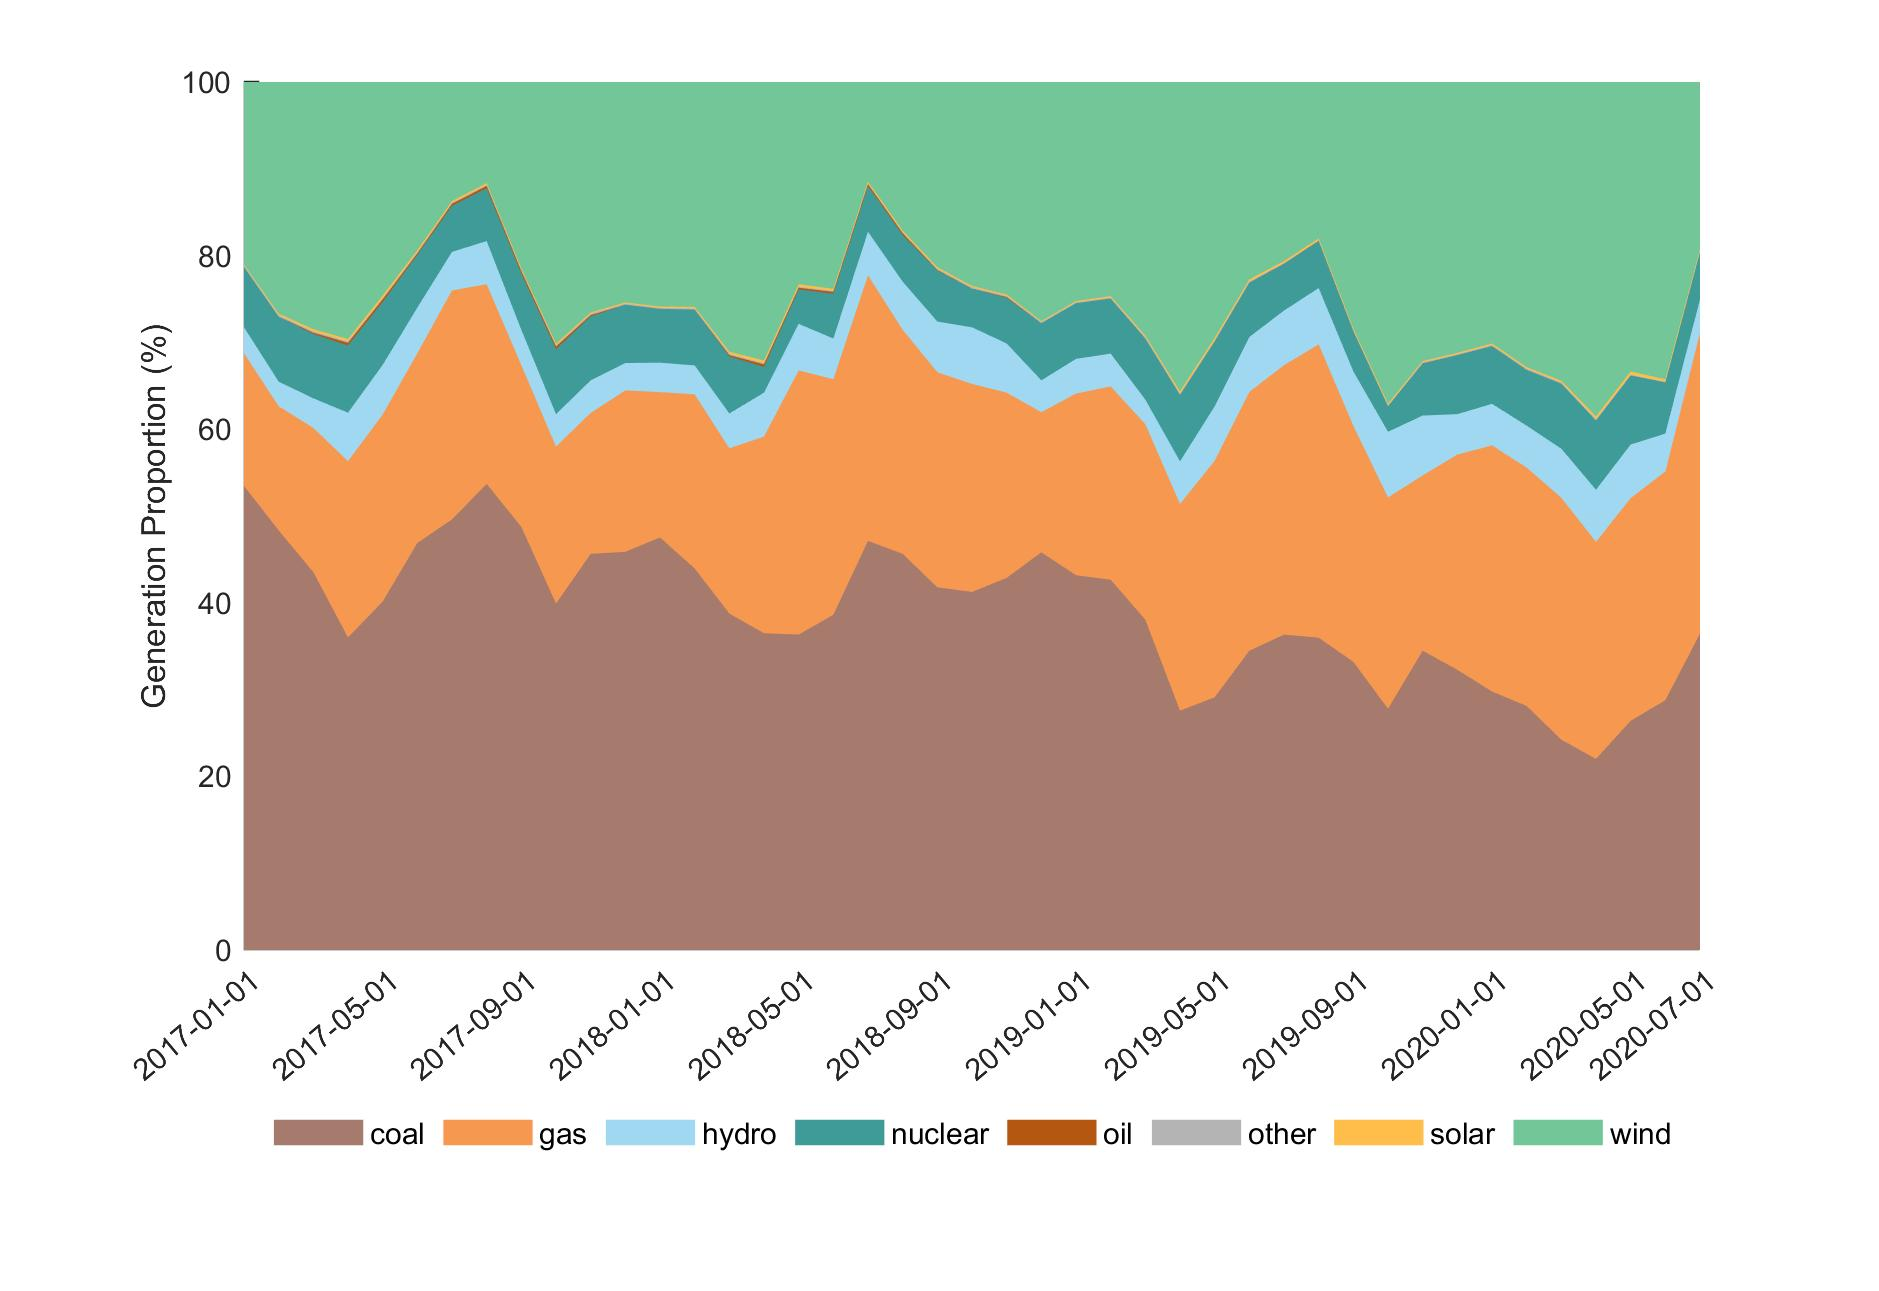
\includegraphics[width=0.8\textwidth]{figures/plot_generation_mix_example1.jpg}
  \caption{Generation Mix of SPP} \label{fig:vis_1}
\end{figure}

And the result is displayed in Figure~\ref{fig:vis_1}. Different color blocks demonstrate different fuel kinds as shown in legends. The area of each block shows the electric generation of each kind of fuel. In this figure, we may see that the main generation structure change is caused by the quantity of wind power generation.
 Additional optional input arguments can be used to set date range and resampling options. Under this circumstance, the arguments should be in the form of name-value pairs. Valid parameter names are listed in Table~\ref{tab:plot_gene_mix_option}. See the help for \verb!plot_generation_mix! for details.
 \newpage

\begin{table}[!ht]
\centering
\begin{threeparttable}
\caption{Plot Generation Mix Option}
\label{tab:plot_gene_mix_option}
\footnotesize
\begin{tabular}{lp{.3\textwidth}p{0.5\textwidth}}
\toprule
Name & Type & Description \\
\midrule
DateRange & \begin{tabular}[t]{l}
datetime array\\
string array\\
cell array of character vectors\\
\end{tabular} & Range of time. \\
& & \begin{tabular}[t]{l @{ -- } l}
Default & \verb!{'2017-01-01','2020-07-15'}!.\\
Example & \verb!{'2017-01-01','2020-07-15'}!\\
& \verb!["2020-02-01","2020-04-30"]!\\
\end{tabular}\\
\midrule
ResampleBin & \begin{tabular}[t]{l}
string\\
character vectors\\
\end{tabular} & Binning scheme for resampling. \tnote{\dag}\\
& & \begin{tabular}[t]{l @{ -- } l}
Default & \verb!'month'!.\\
\end{tabular}\\
\midrule
ColorMap & \begin{tabular}[t]{l}
table\\
structure array\\
string array\\
cell array of character vectors\\
\end{tabular} & Colors of all the areas in the plot. \tnote{\ddag}\\
& & \begin{tabular}[t]{l}
Default --\\
\verb!["coal","gas","oil","nuclear","hydro",!\\
\verb!"wind","solar","other","import";!\\
\verb!"#a67a6d","#f69850","#b35711","#3f9b98",!\\
\verb!"#a0d8f1","#73c698","#ffbd4a",!\\
\verb!"#b4b4b4","white"]!\\
\end{tabular}\\
\midrule
Others & & Modifications of the area objects.\tnote{\ddag}\\
\bottomrule
\end{tabular}
\begin{tablenotes}
    \scriptsize
    \item [\dag] {See also \verb!groupsummary!.}
    \item [\ddag] {See also \verb!Area Properties!.}
\end{tablenotes}
\end{threeparttable}
\end{table}

\subsubsection{plot renewable share}

This function plots the renewable share curve of a market within specified date range. Like \verb!plot!, it returns the line objects of the curve for further modification.

\begin{Code}
  p = plot_renewable_share(market,Name,Value)
\end{Code}

This function is based on \matlab{} function \verb!plot!.

By default, the function plots the renewable share of the specified market from 2017-01-01 to 2020-07-15, with no resampling.Additional optional input arguments can be used to set date range, resampling options and resampling methods. Under this circumstance, the arguments should be in the form of name-value pairs. Valid parameter names are listed in Table~\ref{tab:plot_renewable_share_option}. See the help for \verb!plot_renewable_share! for details.
\clearpage

\begin{table}[!ht]
\centering
\begin{threeparttable}
\caption{Plot Renewable Share Option}
\label{tab:plot_renewable_share_option}
\footnotesize
\begin{tabular}{lp{.3\textwidth}p{0.5\textwidth}}
\toprule
Name & Type & Description \\
\midrule
DateRange & \begin{tabular}[t]{l}
datetime array\\
string array\\
cell array of character vectors\\
\end{tabular} & Range of time. \\
& & \begin{tabular}[t]{l @{ -- } l}
Default & \verb!{'2017-01-01','2020-07-15'}!.\\
Example & \verb!{'2017-01-01','2020-07-15'}!\\
& \verb!["2020-02-01","2020-04-30"]!\\
\end{tabular}\\
\midrule
ResampleBin & \begin{tabular}[t]{l}
string\\
character vectors\\
\end{tabular} & Binning scheme for resampling. \tnote{\dag}\\
& & \begin{tabular}[t]{l @{ -- } l}
Default & \verb!'none'!.\\
\end{tabular}\\
\midrule
      ResampleMethod & \begin{tabular}[t]{l}
        string            \\
        character vectors \\
      \end{tabular} & Computation method for resampling. \tnote{\dag}        \\
                  &                            & \begin{tabular}[t]{l @{ -- } l}
        Default & \verb!'mean'!. \\
      \end{tabular}                         \\
      \midrule
Others & & Modifications of the line objects.\tnote{\ddag}\\
\bottomrule
\end{tabular}
\begin{tablenotes}
    \scriptsize
    \item [\dag] {See also \verb!groupsummary!.}
    \item [\ddag] {See also \verb!Plot Properties!.}
\end{tablenotes}
\end{threeparttable}
\end{table}









\subsection{Demand Profiles}

Electric power demand is a significant aspect of power system analysis. After the COVID-19 outbreak, the features of demand profiles across all U.S. electricity markets have experienced several changes, which offer the researchers an important perspective to analyze the relationship between the epidemic, electricity demand patterns and power system operation.

In \covemda{}, two typical tools regarding different time scales are provided for demand analysis: \verb!plot_demand! and \verb!plot_daily_demand_profile!. Both of them obtain relevant data from file \verb!<market_name>_rto_load.csv! in the data hub.

\subsubsection{plot demand}

This function plots the demand curve of a market within specified date range. Like \verb!plot!, it returns the line object of the curve for further modification.

\begin{Code}
  p = plot_demand(market, varargin);
\end{Code}

This function is based on \matlab{} function \verb!plot!.

By default, the function plots the demand curve of the specified market from 2017-01-01 to 2020-07-15, with no resampling. Additional optional input arguments can be used to set date range and resampling options. Under this circumstance, the arguments should be in the form of name-value pairs. Valid parameter names are listed in Table~\ref{tab:plot_demand_opt}. See the help for \verb!plot_demand! for details.

\begin{table}[!ht]
  \centering
  \begin{threeparttable}
    \caption{Plot Demand Options}
    \label{tab:plot_demand_opt}
    \footnotesize
    \begin{tabular}{lp{.3\textwidth}p{0.5\textwidth}}
      \toprule
      Name        & Type                       & Description                                        \\
      \midrule
      DateRange   & \begin{tabular}[t]{l}
        datetime array                  \\
        string array                    \\
        cell array of character vectors \\
      \end{tabular} & Range of time.                                     \\
                  &                            & \begin{tabular}[t]{l @{ -- } l}
        Default & \verb!{'2017-01-01','2020-07-15'}!. \\
        Example & \verb!{'2017-01-01','2020-07-15'}!  \\
                & \verb!["2020-02-01","2020-04-30"]!  \\
      \end{tabular}                         \\
      \midrule
      ResampleBin & \begin{tabular}[t]{l}
        string            \\
        character vectors \\
      \end{tabular} & Binning scheme for resampling. \tnote{\dag}        \\
                  &                            & \begin{tabular}[t]{l @{ -- } l}
        Default & \verb!'none'!. \\
      \end{tabular}                         \\
      \midrule
      ResampleMethod & \begin{tabular}[t]{l}
        string            \\
        character vectors \\
      \end{tabular} & Computation method for resampling. \tnote{\dag}        \\
                  &                            & \begin{tabular}[t]{l @{ -- } l}
        Default & \verb!'mean'!. \\
      \end{tabular}                         \\
      \midrule
      Others      &                            & Modifications of the line object.\tnote{\ddag}    \\
      \bottomrule
    \end{tabular}
    \begin{tablenotes}
      \scriptsize
      \item [\dag]  {See also \verb!groupsummary!.}
      \item [\ddag] {See also \verb!Line Properties!.}
    \end{tablenotes}
  \end{threeparttable}
\end{table}





\subsubsection{plot daily demand curve}

This function plots the daily demand curve of a market with specified quantiles. It returns all the objects in the plot for further modification. If there are odd quantiles, the central one is displayed as a line object. Otherwise all of them are displayed as area objects.

\begin{Code}
  ar = plot_daily_demand_curve(market, varargin);
\end{Code}

This function is based on \matlab{} function \verb!area! and \verb!plot!.

By default, the function plots the daily demand curve of the specified market from 2017-01-01 to 2020-07-15 with the five quantiles representing its variation: \verb![0.05, 0.25, 0.5, 0.75, 0.95]!. For instance, use the default settings:

\begin{Code}
  >> plot_daily_demand_curve('nyiso');
\end{Code}

\begin{figure}
  \centering
  \noindent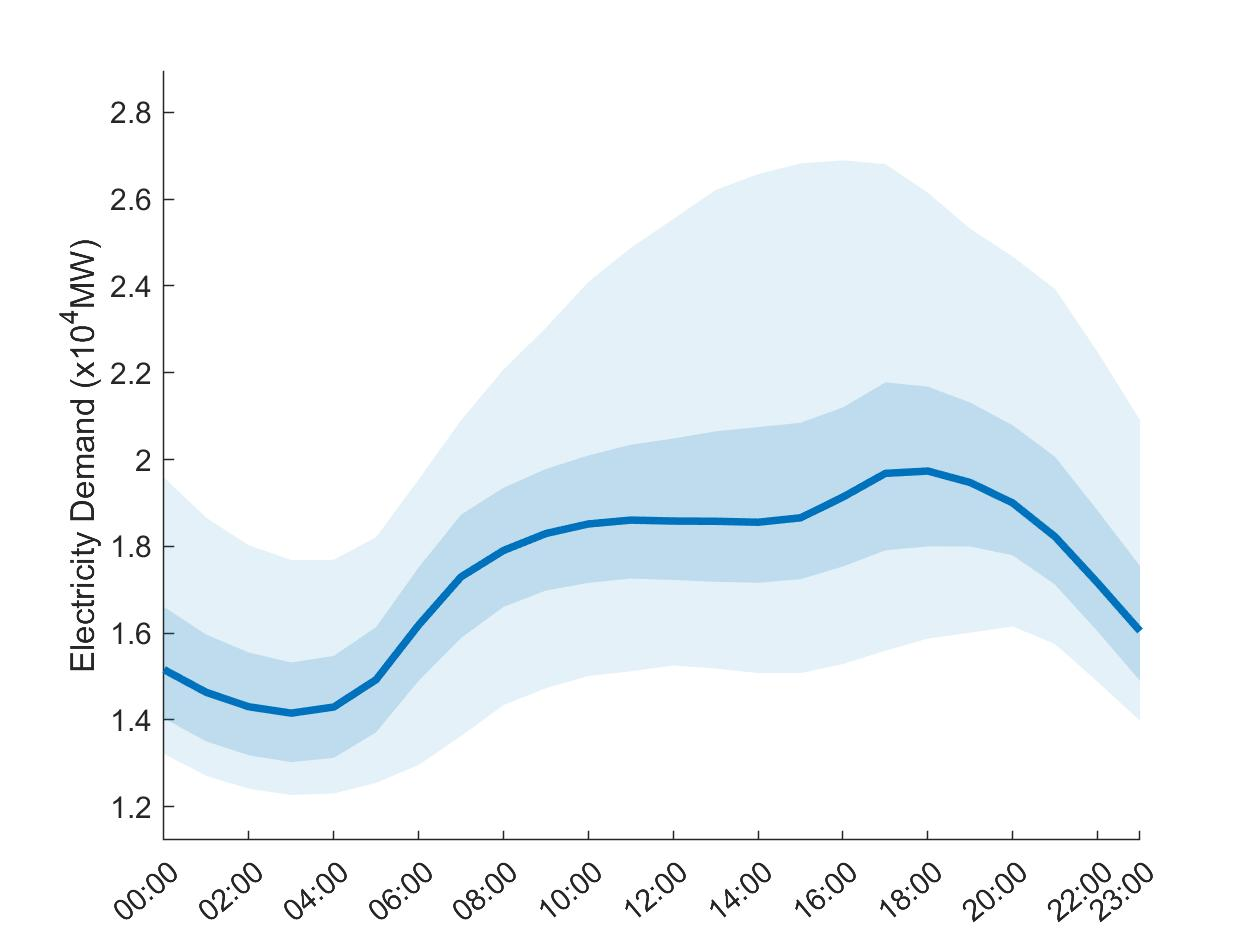
\includegraphics[width=0.8\textwidth]{figures/visualization_plot_daily_demand_curve.jpg}
  \caption{Daily Demand Curve of NYISO} \label{fig:vis_1}
\end{figure}

And the result is displayed in Figure~\ref{fig:vis_1}. In this plot, five edges of color blocks represent the five quantiles, \verb![0.05, 0.25, 0.5, 0.75, 0.95]! successively. As there are odd quantiles, the \verb!0.5! quantile is displayed as the central line. The outer light blue area represents the variation of \verb!0.05~0.95!, and the inner less-light blue area represents \verb!0.25~0.75!, to better illustrate the variation of electricity demand in the date range.

Additional optional input arguments can be used to set date range, quantiles and plot options. Under this circumstance, the arguments should be in the form of name-value pairs. Valid parameter names are listed in Table~\ref{tab:plot_dai_demand_opt}. See the help for \verb!plot_daily_demand_curve! for details.
\clearpage
\begin{table}[!ht]
  \centering
  \begin{threeparttable}
    \caption{Plot Daily Demand Curve Options}
    \label{tab:plot_dai_demand_opt}
    \footnotesize
    \begin{tabular}{lp{.3\textwidth}p{0.5\textwidth}}
      \toprule
      Name        & Type                       & Description                                        \\
      \midrule
      DateRange   & \begin{tabular}[t]{l}
        datetime array                  \\
        string array                    \\
        cell array of character vectors \\
      \end{tabular} & Range of time.                                     \\
                  &                            & \begin{tabular}[t]{l @{ -- } l}
        Default & \verb!{'2017-01-01','2020-07-15'}!. \\
        Example & \verb!{'2017-01-01','2020-07-15'}!  \\
                & \verb!["2020-02-01","2020-04-30"]!  \\
      \end{tabular}                         \\
      \midrule
      Quantile   & \begin{tabular}[t]{l}
        numeric vector                  \\
      \end{tabular} & Cumulative probabilities. \tnote{\dag}  \\
                  &                            & \begin{tabular}[t]{l @{ -- } l}
        Default & \verb![0.05, 0.25, 0.5, 0.75, 0.95]!. \\
      \end{tabular}                         \\
      \midrule
      Color & \begin{tabular}[t]{l}
        RGB triplet \\
        hexadecimal color code \dots  \\
      \end{tabular} & Color theme of the plot.        \\
                  &                            & \begin{tabular}[t]{l @{ -- } l}
        Default & \verb!'#0072BD'!. \\
      \end{tabular}                         \\
      \midrule
      Alpha & \begin{tabular}[t]{l}
        numeric vector            \\
      \end{tabular} & Face transparency of the objects.        \\
                  &                            & \begin{tabular}[t]{l @{ -- } l}
        Default & \verb![0.1, 0.25]!. \\
      \end{tabular}                         \\
      \midrule
      LineWidth & \begin{tabular}[t]{l}
        positive value            \\
      \end{tabular} & Width of the central line (if exists).       \\
                  &                            & \begin{tabular}[t]{l @{ -- } l}
        Default & \verb!2.5!. \\
      \end{tabular}                         \\
      \midrule
      Others      &      & Modifications of the area objects. \tnote{\ddag}    \\
      \bottomrule
    \end{tabular}
    \begin{tablenotes}
      \scriptsize
      \item [\dag]  {See also \verb!quantile!.}
      \item [\ddag] {See also \verb!Area Properties!.}
    \end{tablenotes}
  \end{threeparttable}
\end{table}





\subsection{Price Distribution}

In this section, we provide two typical tools to display the electricity price in U.S.  After the COVID-19 outbreak, electricity price become harder to trace. In order to trace the change of electricity price, we may observe the price data of different markets in U.S. and organize them into plots. This may offer a new approach for researchers to find out the structure change of U.S. power grid brought by COVID-19.

In \covemda{}, two typical tools regarding different scales are provided for price analysis: \verb!plot_price! and \verb!plotprice_distribution!. Both of them obtain relevant data from file \verb!<market_name>_rto_lmp.csv! in the data hub.

\subsubsection{plot price}

This function plots the price curve of a market within specified date range. Like \verb!plot!, it returns the line objects of the curve for further modification.

\begin{Code}
  p = plot_price(market,Name,Value)
\end{Code}

This function is based on \matlab{} function \verb!plot!.

By default, the function plots the price of the specified market from 2017-01-01 to 2020-07-15, with no resampling.Additional optional input arguments can be used to set date range, resampling options and resampling methods. Under this circumstance, the arguments should be in the form of name-value pairs. Valid parameter names are listed in Table~\ref{tab:plot_price_option}. See the help for \verb!plot_price! for details.

\begin{table}[!ht]
\centering
\begin{threeparttable}
\caption{Plot Price Option}
\label{tab:plot_price_option}
\footnotesize
\begin{tabular}{lp{.3\textwidth}p{0.5\textwidth}}
\toprule
Name & Type & Description \\
\midrule
DateRange & \begin{tabular}[t]{l}
datetime array\\
string array\\
cell array of character vectors\\
\end{tabular} & Range of time. \\
& & \begin{tabular}[t]{l @{ -- } l}
Default & \verb!{'2017-01-01','2020-07-15'}!.\\
Example & \verb!{'2017-01-01','2020-07-15'}!\\
& \verb!["2020-02-01","2020-04-30"]!\\
\end{tabular}\\
\midrule
ResampleBin & \begin{tabular}[t]{l}
string\\
character vectors\\
\end{tabular} & Binning scheme for resampling. \tnote{\dag}\\
& & \begin{tabular}[t]{l @{ -- } l}
Default & \verb!'none'!.\\
\end{tabular}\\
\midrule
      ResampleMethod & \begin{tabular}[t]{l}
        string            \\
        character vectors \\
      \end{tabular} & Computation method for resampling. \tnote{\dag}        \\
                  &                            & \begin{tabular}[t]{l @{ -- } l}
        Default & \verb!'mean'!. \\
      \end{tabular}                         \\
      \midrule
Others & & Modifications of the line objects.\tnote{\ddag}\\
\bottomrule
\end{tabular}
\begin{tablenotes}
    \scriptsize
    \item [\dag] {See also \verb!groupsummary!.}
    \item [\ddag] {See also \verb!Plot Properties!.}
\end{tablenotes}
\end{threeparttable}
\end{table}

\subsubsection{plot price distribution}

This function plots the price distribution of a market. 

\begin{Code}
  ar = plot_price_distribution(market, Name, Value);
\end{Code}

This function is based on \matlab{} function \verb!plot!.

By default, the function plots the price distribution of the specified market from 2017-01-01 to 2020-07-15. For instance, use the default settings:

\begin{Code}
  >> plot_price_distribution('isone');
\end{Code}

\begin{figure}
  \centering
  \noindent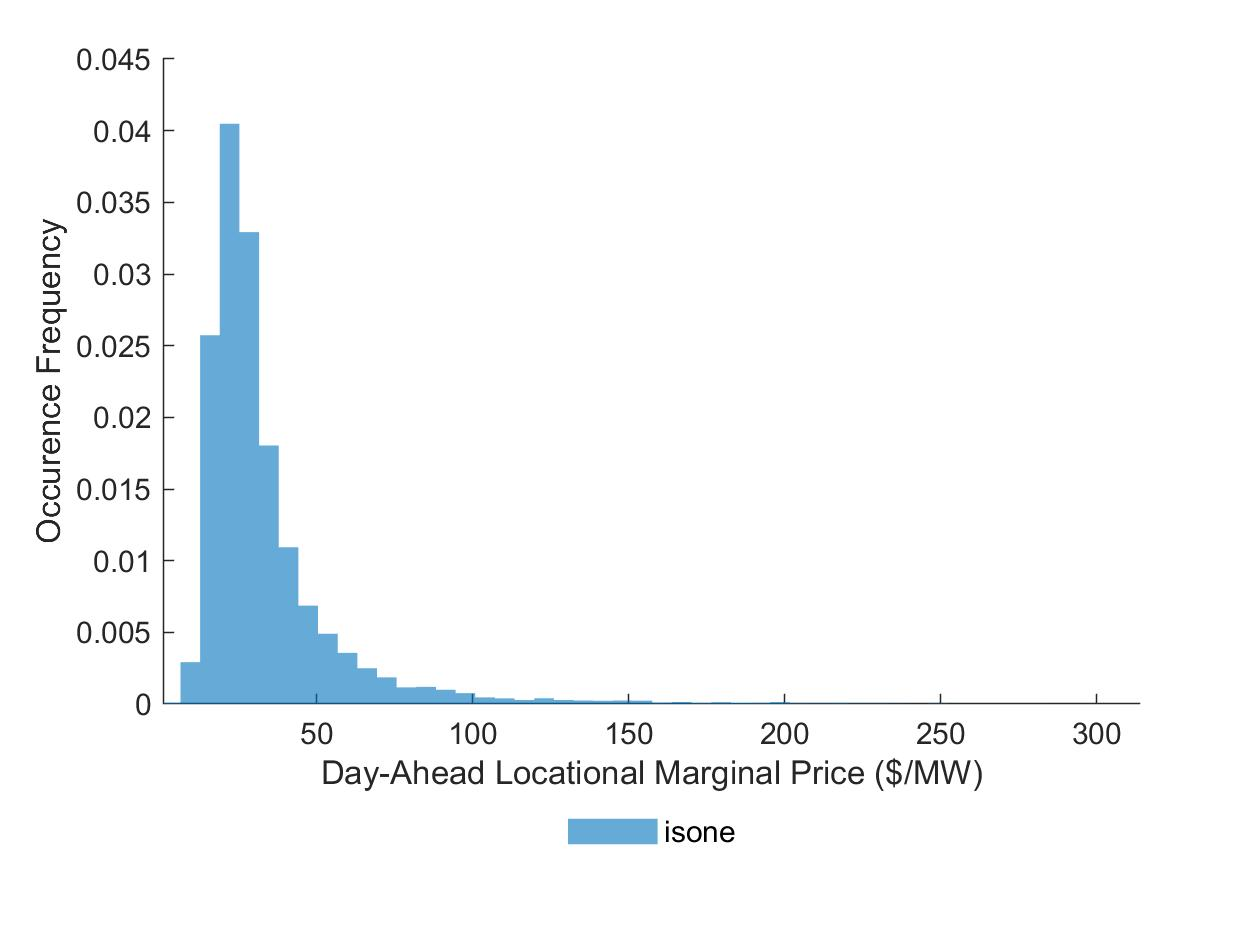
\includegraphics[width=0.8\textwidth]{figures/visualization_example1.jpg}
  \caption{Price Distribution of ISONE} \label{fig:vis_1}
\end{figure}

And the result is displayed in Figure~\ref{fig:vis_1}. 

Additional optional input arguments can be used to set date range and other options. Under this circumstance, the arguments should be in the form of name-value pairs. Valid parameter names are listed in Table~\ref{tab:plot_price_distribution_opt}. See the help for \verb!plot_price_distribution! for details.
\clearpage
\begin{table}[!ht]
  \centering
  \begin{threeparttable}
    \caption{Plot Price Distribution Options}
    \label{tab:plot_price_distribution_opt}
    \footnotesize
    \begin{tabular}{lp{.3\textwidth}p{0.5\textwidth}}
      \toprule
      Name        & Type                       & Description                                        \\
      \midrule
      DateRange   & \begin{tabular}[t]{l}
        datetime array                  \\
        string array                    \\
        cell array of character vectors \\
      \end{tabular} & Range of time.                                     \\
                  &                            & \begin{tabular}[t]{l @{ -- } l}
        Default & \verb!{'2017-01-01','2020-07-15'}!. \\
        Example & \verb!{'2017-01-01','2020-07-15'}!  \\
                & \verb!["2020-02-01","2020-04-30"]!  \\
      \end{tabular}                         \\
      \midrule
      Others      &      & Modifications of the histogram objects. \tnote{\dag}    \\
      \bottomrule
    \end{tabular}
    \begin{tablenotes}
      \scriptsize
      \item [\dag] {See also \verb!Histogram Properties!.}
    \end{tablenotes}
  \end{threeparttable}
\end{table}

\subsection{Mobility}

Mobility is a factor directly related with the pandemic. Here 'mobility' means the number of visits to business premises, indicating the level of commercial activities. During COVID-19, the mobility in various sectors have experienced dramatic reduction, which is one of the first signals of the outbreak.

In \covemda{}, the mobility data for three sectors are provided: \verb!Restaurant_Recreation!, \verb!Grocery_Pharmacy! and \verb!Retail!. Unlike other functions in this section, here the data are focused on \textbf{seven major cities}: Los Angeles(\verb!la!), Houston(\verb!houston!), Boston(\verb!boston!), New York City(\verb!nyc!), Chicago(\verb!chicago!), Philadelphia(\verb!phila!) and Kansas City(\verb!kck!). All the data above are obtained from file \verb!<market_name>_<city_name>_patterns.csv! and can be visualized by function \verb!plot_mobility!.

\subsubsection{plot mobility}

This function plots the appointed mobility curve of one of the seven cities. Like \verb!plot!, it returns the line object of the curve for further modification.

\begin{Code}
  p = plot_mobility(city, varargin);
\end{Code}

This function is based on \matlab{} function \verb!plot!.

By default, the function plots the mobility data of the retail sector in the specified city from 2019-12-30 to 2020-11-22, with no resampling. Additional optional input arguments can be used to set sector, date range and resampling options. Under this circumstance, the arguments should be in the form of name-value pairs. Valid parameter names are listed in Table~\ref{tab:plot_mob_opt}. See the help for \verb!plot_mobility! for details.

\begin{table}[!ht]
  \centering
  \begin{threeparttable}
    \caption{Plot Mobility Options}
    \label{tab:plot_mob_opt}
    \footnotesize
    \begin{tabular}{lp{.3\textwidth}p{0.5\textwidth}}
      \toprule
      Name        & Type                       & Description                                        \\
      \midrule
      DateRange   & \begin{tabular}[t]{l}
        datetime array                  \\
        string array                    \\
        cell array of character vectors \\
      \end{tabular} & Range of time.                                     \\
                  &                            & \begin{tabular}[t]{l @{ -- } l}
        Default & \verb!{'2017-01-01','2020-07-15'}!. \\
        Example & \verb!{'2017-01-01','2020-07-15'}!  \\
                & \verb!["2020-02-01","2020-04-30"]!  \\
      \end{tabular}                         \\
      \midrule
      Sector & \begin{tabular}[t]{l}
        string            \\
        character vectors \\
      \end{tabular} & The sector to be plotted.        \\
                  &                            & \begin{tabular}[t]{l @{ -- } l}
        Default & \verb!'Retail'!. \\
        Example & \verb!'Retail'!. \\
                & \verb!'Restaurant_Recreaction'! \\
                & \verb!'Grocery_Pharmacy'!       \\
      \end{tabular}                         \\
      \midrule
      ResampleBin & \begin{tabular}[t]{l}
        string            \\
        character vectors \\
      \end{tabular} & Binning scheme for resampling. \tnote{\dag}        \\
                  &                            & \begin{tabular}[t]{l @{ -- } l}
        Default & \verb!'none'!. \\
      \end{tabular}                         \\
      \midrule
      ResampleMethod & \begin{tabular}[t]{l}
        string            \\
        character vectors \\
      \end{tabular} & Computation method for resampling. \tnote{\dag}        \\
                  &                            & \begin{tabular}[t]{l @{ -- } l}
        Default & \verb!'mean'!. \\
      \end{tabular}                         \\
      \midrule
      Others      &                            & Modifications of the line object.\tnote{\ddag}    \\
      \bottomrule
    \end{tabular}
    \begin{tablenotes}
      \scriptsize
      \item [\dag]  {See also \verb!groupsummary!.}
      \item [\ddag] {See also \verb!Line Properties!.}
    \end{tablenotes}
  \end{threeparttable}
\end{table}





\subsection{Examples}

\subsubsection{Basic Usage} \label{subsubsec:vis_basic}

All functions mentioned above have similar input-output forms and can be used similarly. To be specific, the first input argument (market name or city name) is complimentary, and all the other input arguments are optional. The market name is specified as one of the seven terms:

\begin{center}
  \verb!'caiso' | 'ercot' | 'isone' | 'miso' | 'nyiso' | 'pjm' | 'spp'!
\end{center}

And the city name is specified as one of the seven abbreviations:

\begin{center}
  \verb!'la' | 'houston' | 'boston' | 'nyc' | 'chicago' | 'phila' | 'kck'!
\end{center}

For \verb!plot_mobility! where the city name needs to be specified, the corresponding market name is not necessary. The function automatically recognizes the market which the city is in, as long as it is one of the seven cities listed above.

All the other input arguments should be in the form of \textbf{name-value pairs} for the function to correctly recognize.

\begin{Code}
  plot_demand(market, 'argument_name1', argument_value1,
  'argument_name2', argument_value2, ...);
\end{Code}

Valid parameter names for each function above are listed in Table~\ref{tab:plot_gene_mix_option} to \ref{tab:plot_mob_opt}. Pay attention that \verb!plot_demand!, \verb!plot_renewable_share!, \verb!plot_price! and \verb!plot_mobility! are based on \matlab{} function \verb!plot!, \verb!plot_generation_mix! is based on \verb!area! and \verb!plot_price_distribution! based on \verb!histogram!. For those functions, all the name-value pair arguments are passed to corresponding \matlab{} functions except the ones listed in the table. For \verb!plot_daily_demand_curve!, however, the arguments are mainly passed to \verb!area!. If there are odd quantiles, the central one is displayed with \verb!plot! and only \verb!'Color'! and \verb!'LineWidth'! are passed to it.

The output argument is the graphics object(s) of the plot, just like \verb!plot!, \verb!area! and \verb!histogram!. The number of the object depends on the function type. For \verb!plot_renewable_share!, \verb!plot_demand!, \verb!plot_price! and \verb!plot_mobility!, the function returns only one line object. For \verb!plot_generation_mix!, the number of area objects returned is equal to the number of fuel types. For \verb!plot_price_distribution!, the function returns only one histogram object. For \verb!plot_daily_demand_curve!, the function returns all the area objects and the line object (if exists) of the plot. It can be utilized to modify the plot after calling the function, as is illustrated in \ref{subsubsec:vis_cus}.

As long as the market name (or the city name) is given, a basic version of the desired plot can be simply obtained. For example, to plot the price distribution histogram of ISONE, just enter

\begin{Code}
  >> plot_price_distribution('isone');
\end{Code}

\begin{figure}
  \centering
  \noindent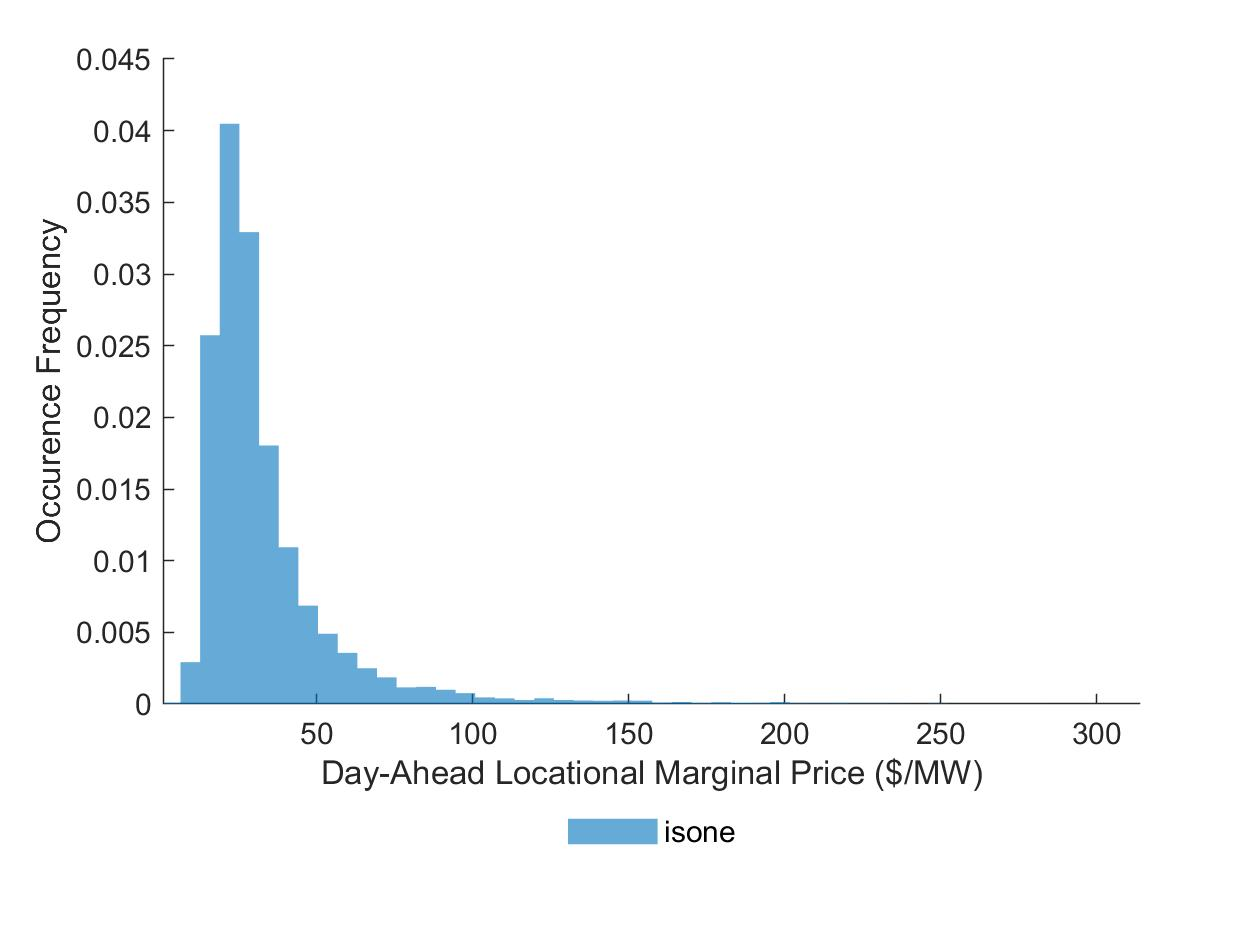
\includegraphics[width=0.8\textwidth]{figures/visualization_example1.jpg}
  \caption{Example: Price Distribution of ISONE} \label{fig:vis_eg1}
\end{figure}

The result is displayed in Figure~\ref{fig:vis_eg1}. By default, the price distribution histogram of ISONE from 2017-01-01 to 2020-07-15 is plotted. If the user wants to change the date range, parameter \verb!DateRange! should be specified. For example, to plot the renewable share curve of NYISO from February to April in 2020, the user may enter

\begin{Code}
  >> plot_renewable_share('nyiso', 'DateRange', {'2020-02-01',
      '2020-04-30'});
\end{Code}

\begin{figure}
  \centering
  \noindent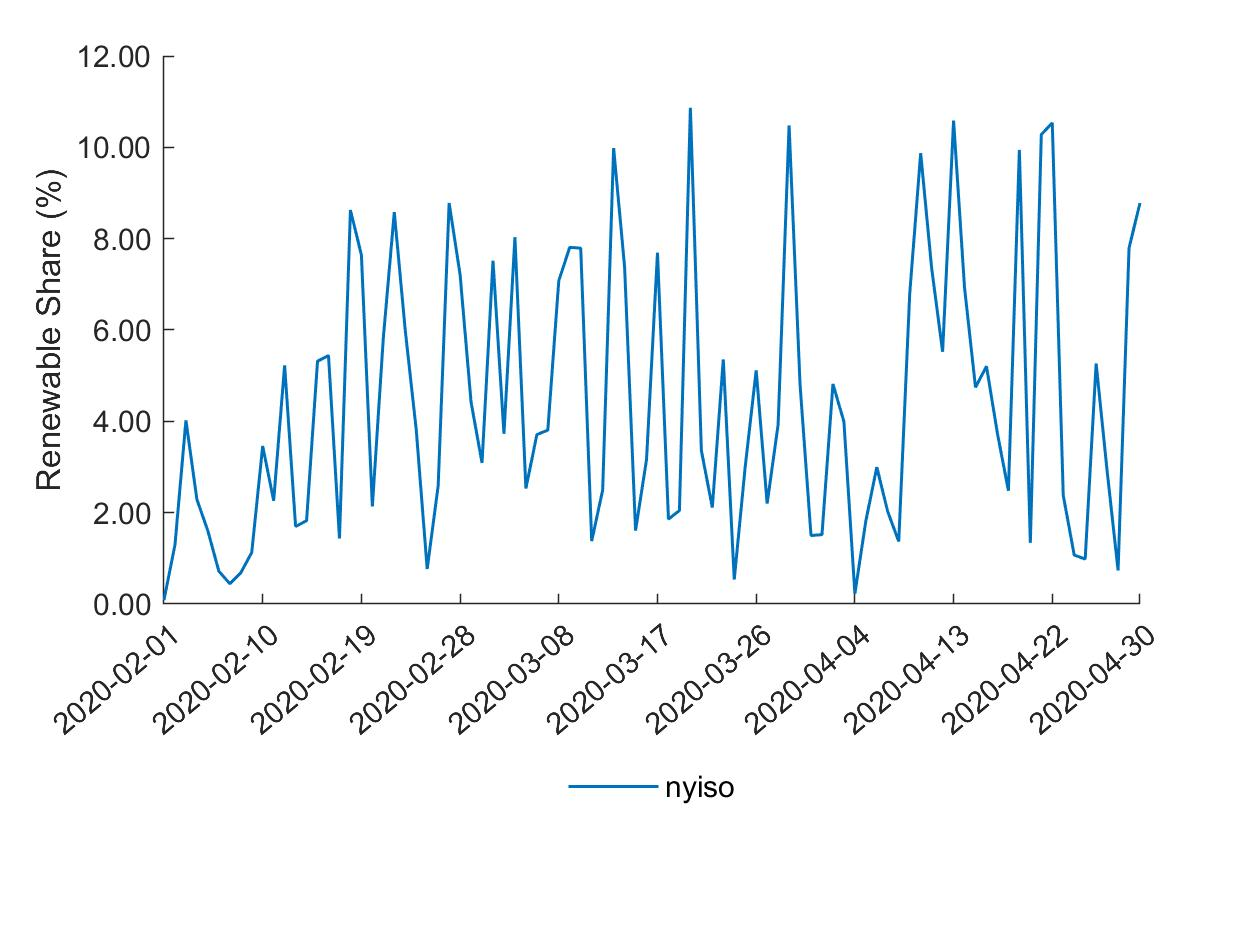
\includegraphics[width=0.8\textwidth]{figures/visualization_example2.jpg}
  \caption{Example: Renewable Share of NYISO} \label{fig:vis_eg2}
\end{figure}

The result is displayed in Figure~\ref{fig:vis_eg2}, where the desired renewable share curve is plotted.

Some of the functions provide an option for resampling data, making them more flexible to use. For example, to plot the average price of every month in 2019, the user may enter

\begin{Code}
  >> plot_price('nyiso', 'DateRange', {'2019-01-01', '2019-12-31'},
  'ResampleBin', 'month', 'ResampleMethod', 'mean');
\end{Code}

\begin{figure}
  \centering
  \noindent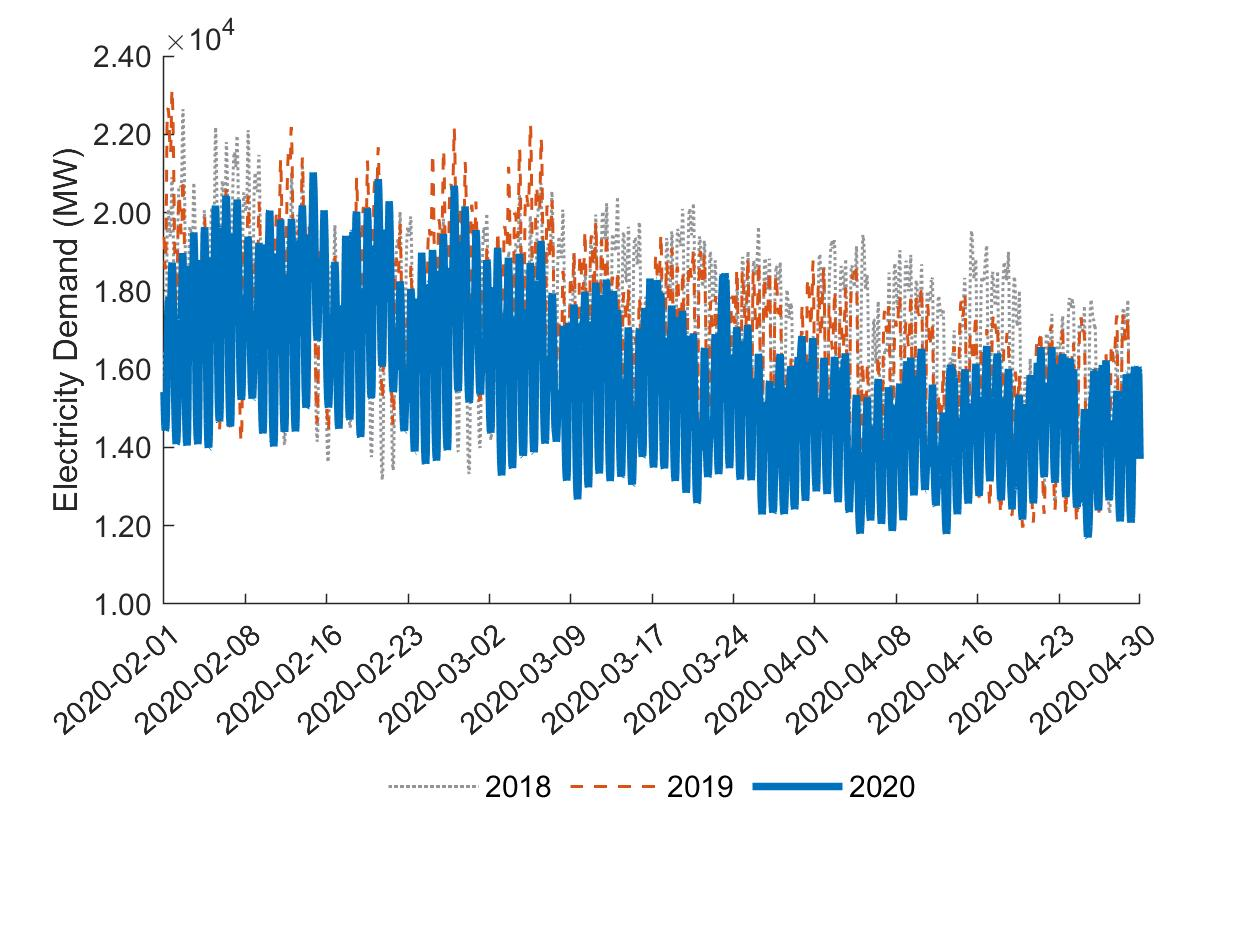
\includegraphics[width=0.8\textwidth]{figures/visualization_example3.jpg}
  \caption{Example: Average Price of NYISO} \label{fig:vis_eg3}
\end{figure}

The result is displayed in Figure~\ref{fig:vis_eg3}, where the desired price trend is plotted.

Like \verb!plot!, all the functions can be used more than once to plot multiple curves in one figure. For example, to plot the demand curves of NYISO in 2018, 2019 and 2020 with week alignment, first calculate the corresponding date range:

\begin{Code}
  >> dr_2020 = datetime({'2020-02-01', '2020-04-30'});
  >> dw = calweeks(52);
  >> dr_2019 = dr_2020 - dw;
  >> dr_2018 = dr_2019 - dw;
\end{Code}

Thus the desired date ranges for 2018, 2019 and 2020 are \verb!dr_2018!, \verb!dr_2019! and \verb!dr_2020! correspondingly. Now plot the demand curves:

\begin{Code}
  >> plot_demand('nyiso', 'DateRange', dr_2018, 'DisplayName',
  '2018', 'LineStyle', ':', 'Color', '#939598');
  >> plot_demand('nyiso', 'DateRange', dr_2019, 'DisplayName',
  '2019', 'LineStyle', '--', 'Color', '#D95319');
  >> plot_demand('nyiso', 'DateRange', dr_2020, 'DisplayName',
  '2020', 'Color', '#0072BD', 'LineWidth', 2.5);
\end{Code}

\begin{figure}
  \centering
  \noindent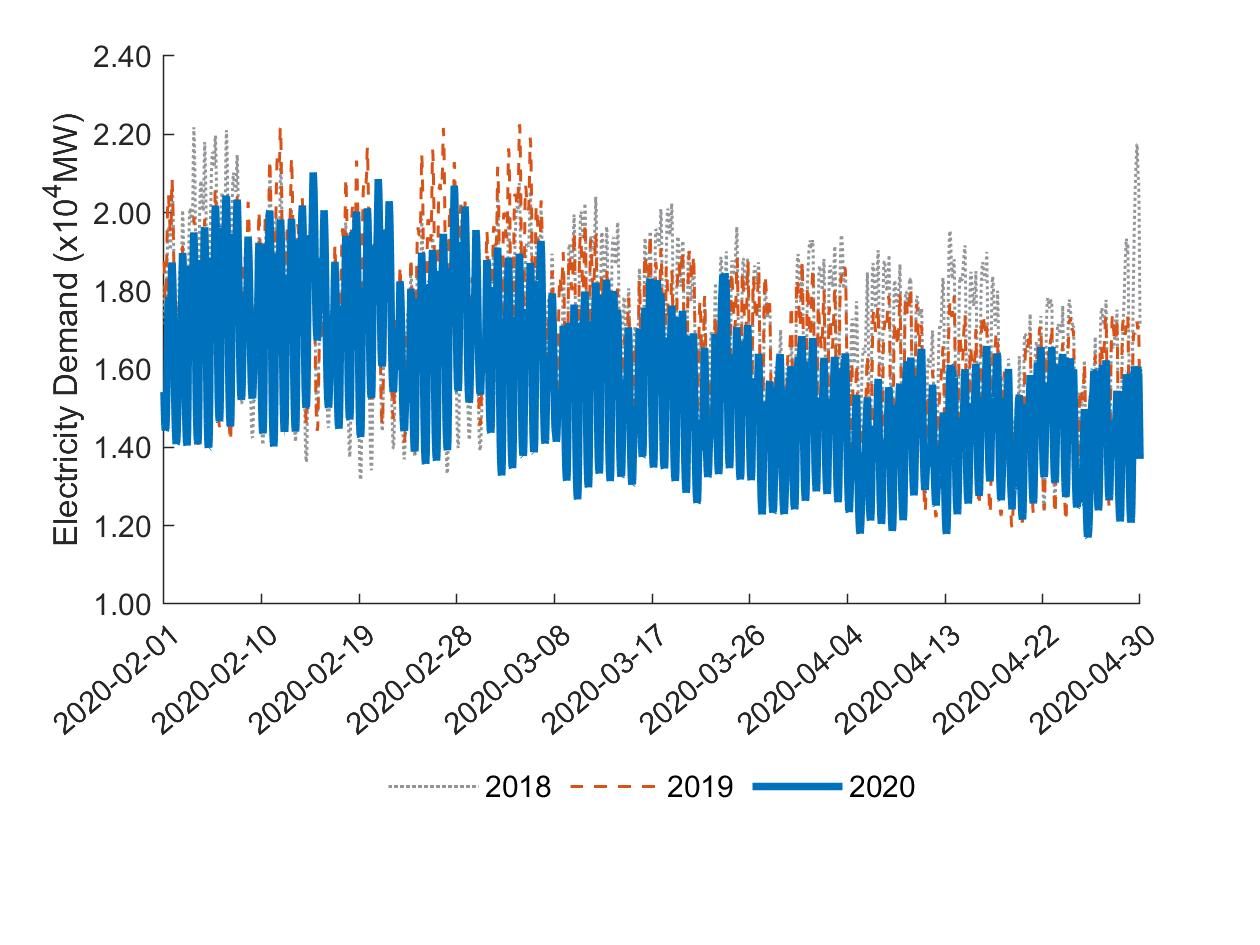
\includegraphics[width=0.8\textwidth]{figures/visualization_example4.jpg}
  \caption{Example: Demand Curves of NYISO} \label{fig:vis_eg4}
\end{figure}

The result is displayed in Figure~\ref{fig:vis_eg4}, where the desired demand curves are plotted. In the example above, several properties of the lines are customized for better recognition. In \ref{subsubsec:vis_cus}, the modification of plots is explored further.



\subsubsection{Customize Plot Properties} \label{subsubsec:vis_cus}

Like \matlab{}, there are mainly two approaches in \covemda{} to modifying a plot: before and after calling the plotting function. The former way refers to passing arguments in the form of \textbf{name-value pairs}, and the latter one refers to changing \textbf{property values} of the chart. They each have their own strengths, and both of them are commonly used to beautify a plot.

In the last example in \ref{subsubsec:vis_basic}, several properties (label, color and line width) of the three lines are modified by passing name-value pair arguments to the function. In this way, the user is able to integrate multiple modifications in one line of code, making it concise and simple. For example, to display markers at data points, the user may enter

\begin{Code}
  >> plot_price('nyiso', 'ResampleBin', 'month', 'Marker', 'o');
\end{Code}

\begin{figure}
  \centering
  \noindent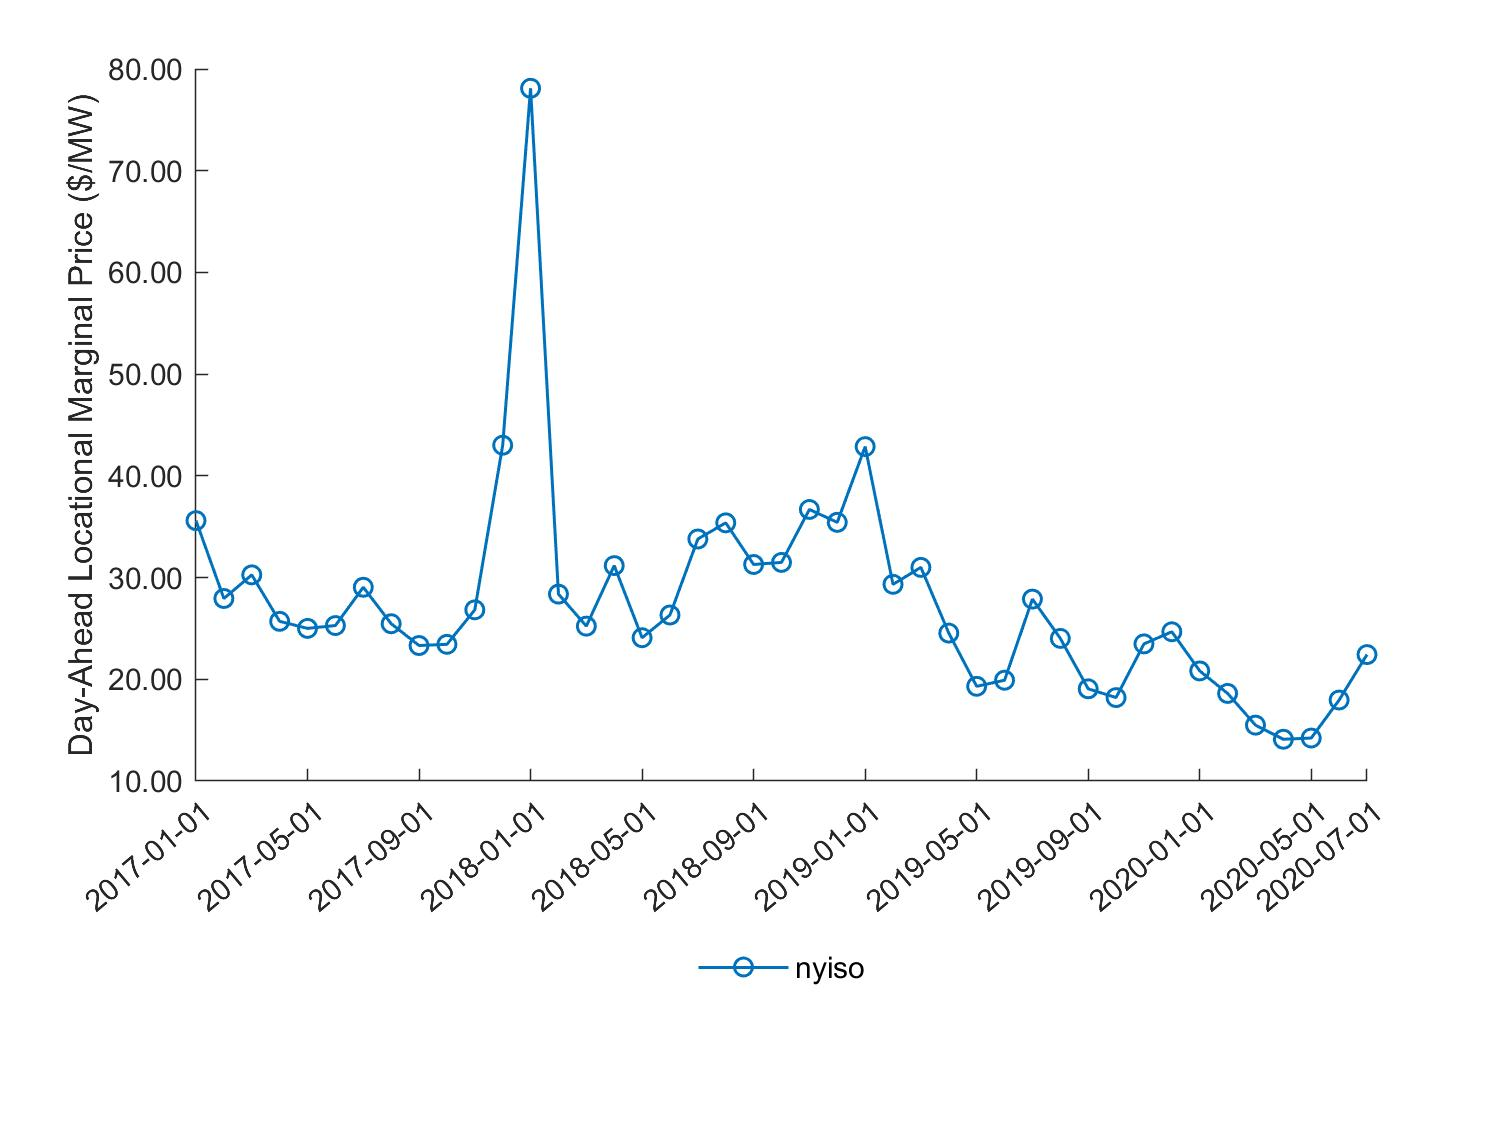
\includegraphics[width=0.8\textwidth]{figures/visualization_example5.jpg}
  \caption{Example: Average Price of NYISO (with Markers)} \label{fig:vis_eg5}
\end{figure}

The result is displayed in Figure~\ref{fig:vis_eg5}, where all the data points are marked with a symbol 'o'. Any other marker symbol can be used in the same way, as long as it is recognized by \verb!plot!.

However, it is difficult to obtain detailed control of the plot by merely passing arguments to the functions, which is why sometimes we also need to change property values after plotting the figure. For example, to change the default display range of y-axis, the user may enter

\begin{Code}
  >> plot_daily_demand_curve('nyiso');
  >> ax = gca;
  >> ax.YLim = [0, 4];
\end{Code}

\begin{figure}
  \centering
  \noindent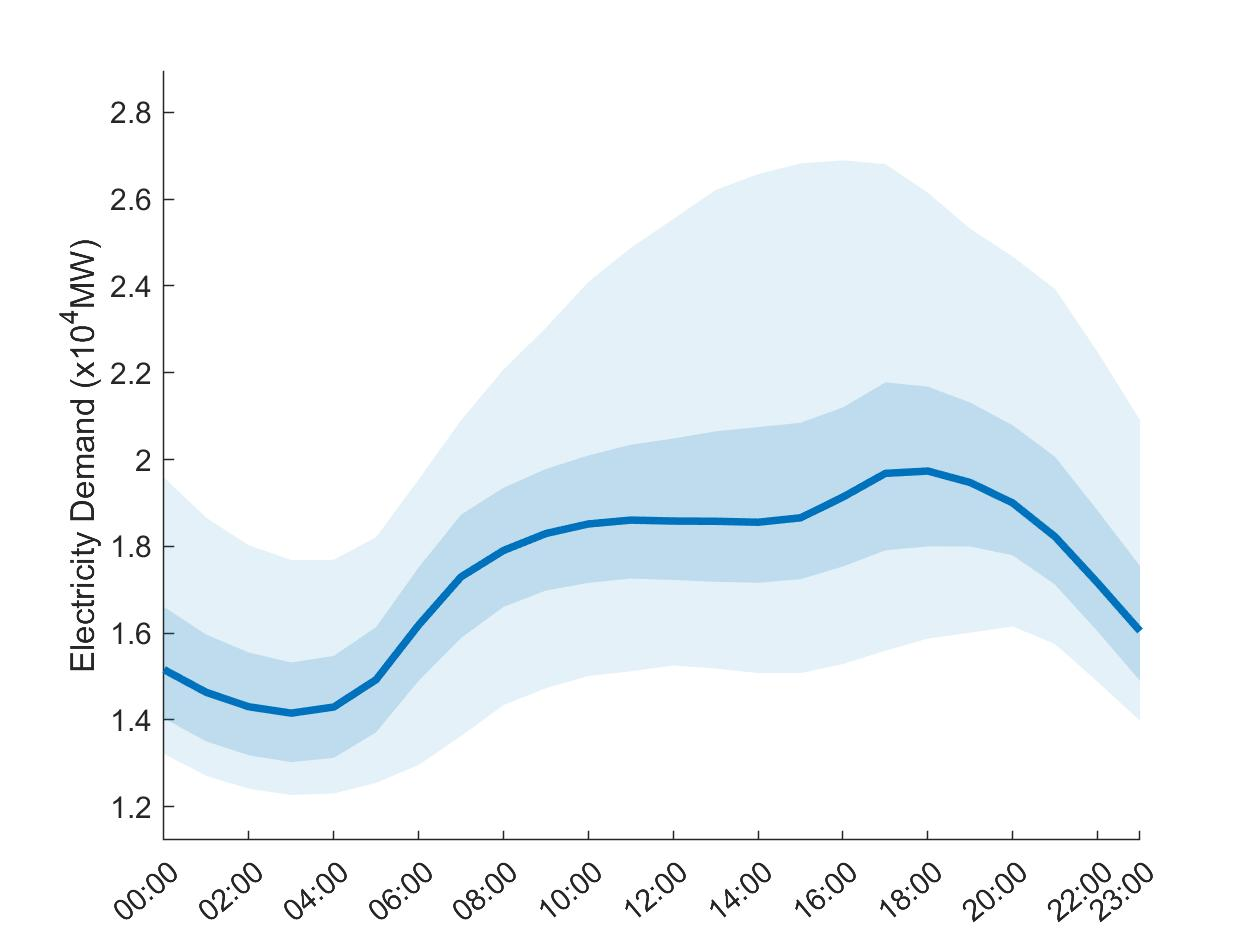
\includegraphics[width=0.8\textwidth]{figures/visualization_example6_1.jpg}
  \caption{Example: Daily Demand Curve of NYISO (Before Changing range of y-axis)} \label{fig:vis_eg6_1}
\end{figure}

\begin{figure}
  \centering
  \noindent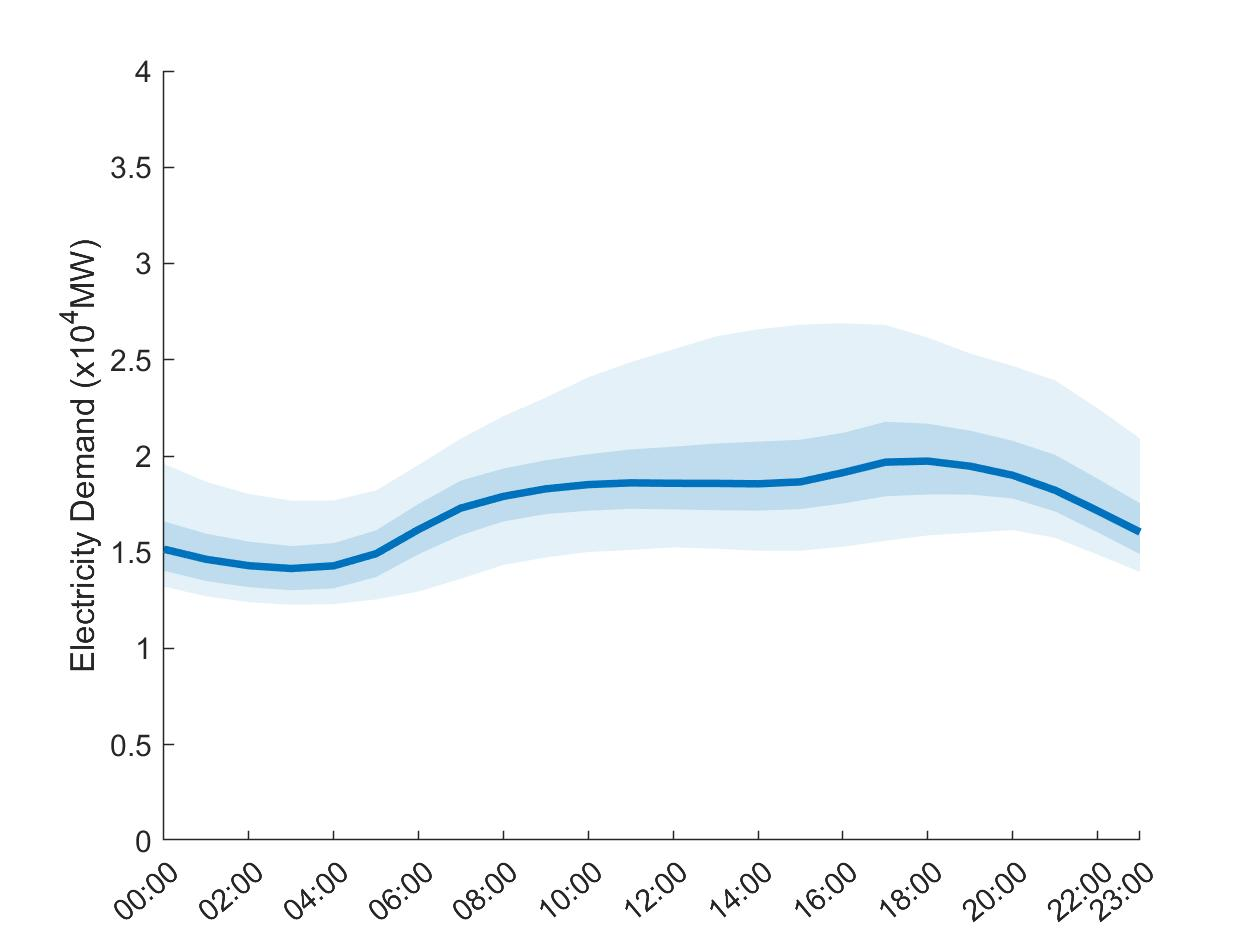
\includegraphics[width=0.8\textwidth]{figures/visualization_example6_2.jpg}
  \caption{Example: Daily Demand Curve of NYISO (After Changing range of y-axis)} \label{fig:vis_eg6_2}
\end{figure}

The result is displayed in Figure~\ref{fig:vis_eg6_1} and \ref{fig:vis_eg6_2}, where the range of y-axis is enlarged. As the modified property belongs to the axes of the figure rather than area or line objects, the command \verb!ax = gca! is utilized to access the axes. Also, \verb!ylim([0, 4])! (using the function \verb!ylim!) has the same effect as \verb!ax.YLim = [0, 4]! in this case.

Under some circumstances, there may exist more than one object in the graph, which is common when using functions concerning \verb!area!. For example, to highlight renewable energy in a generation mix graph, the user may enter

\begin{Code}
  >> ar = plot_generation_mix('spp');
  >> ar(1).FaceColor = '#868686';
  >> ar(2).FaceColor = '#acacac';
  >> ar(4).FaceColor = '#7f7f7f';
  >> ar(5).FaceColor = '#6b6b6b';
\end{Code}

\begin{figure}
  \centering
  \noindent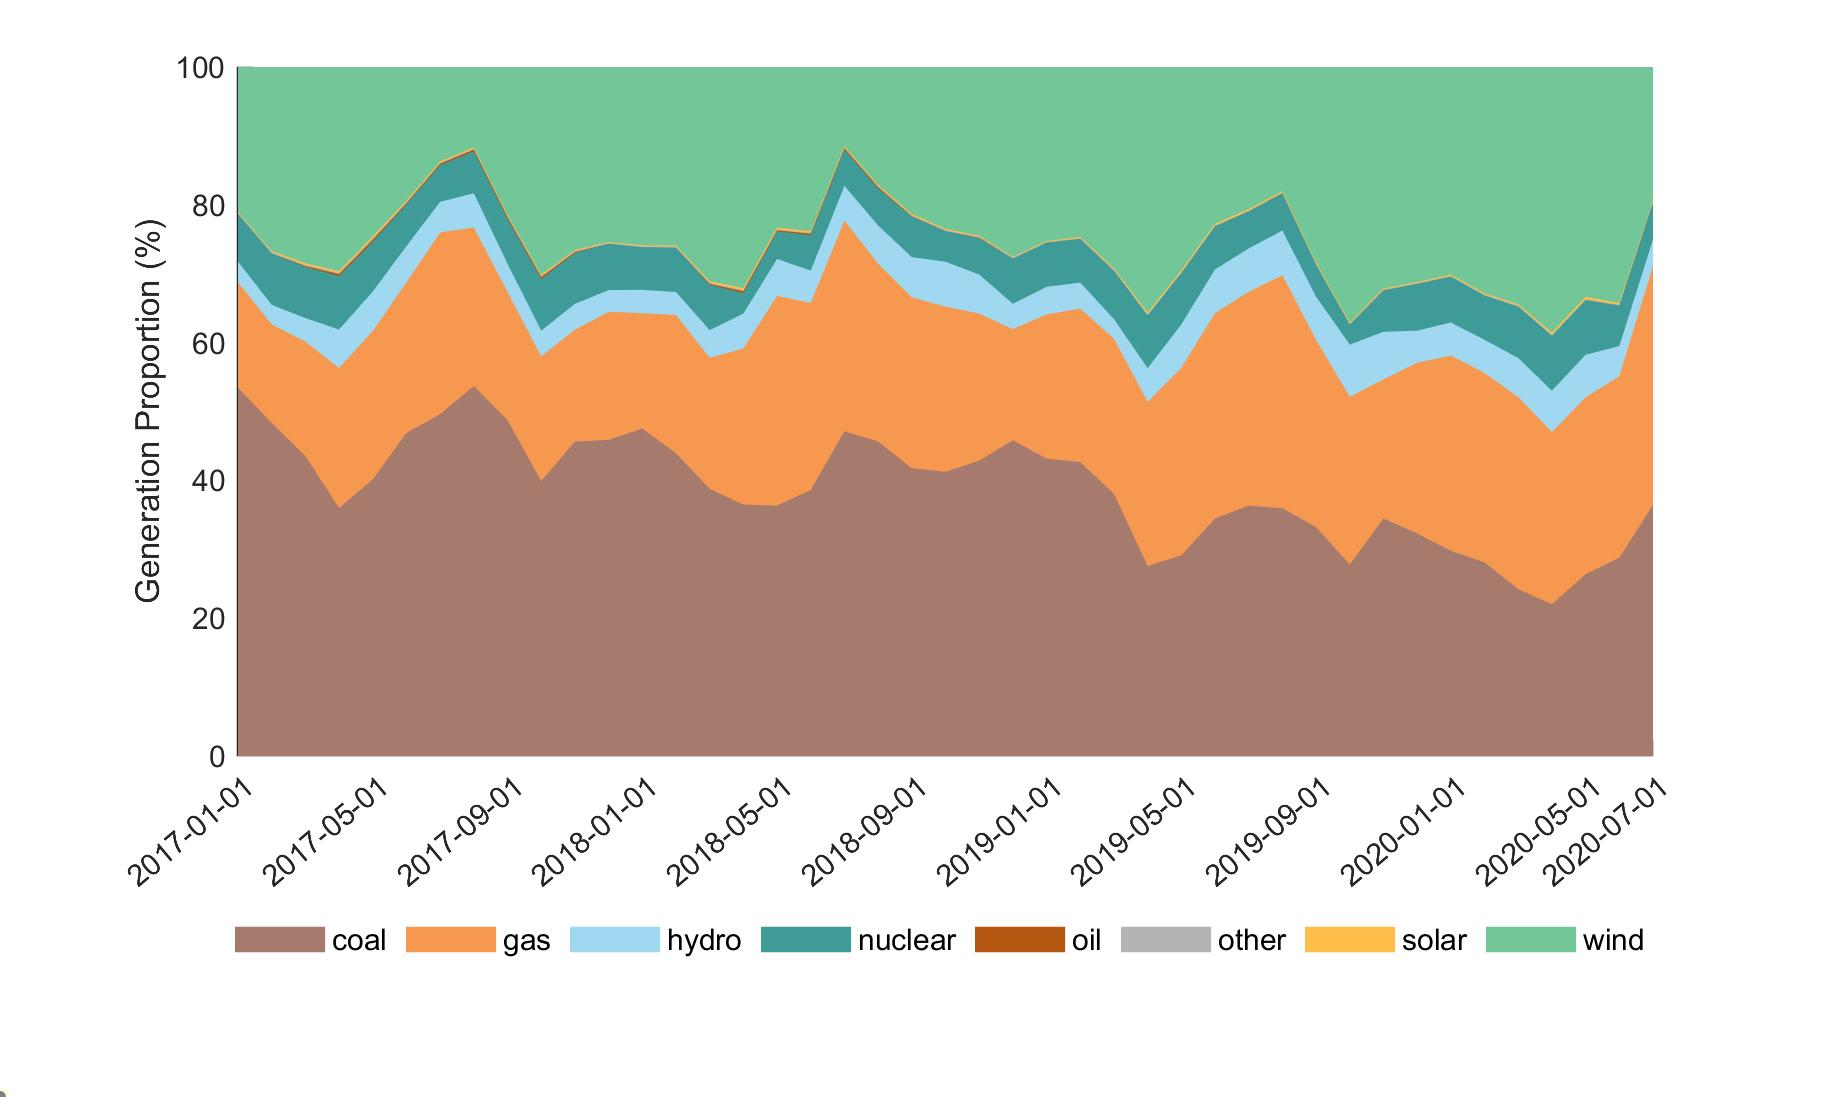
\includegraphics[width=0.8\textwidth]{figures/visualization_example7_1.jpg}
  \caption{Example: Generation Mix of SPP (Before Highlighting Renewables)} \label{fig:vis_eg7_1}
\end{figure}

\begin{figure}
  \centering
  \noindent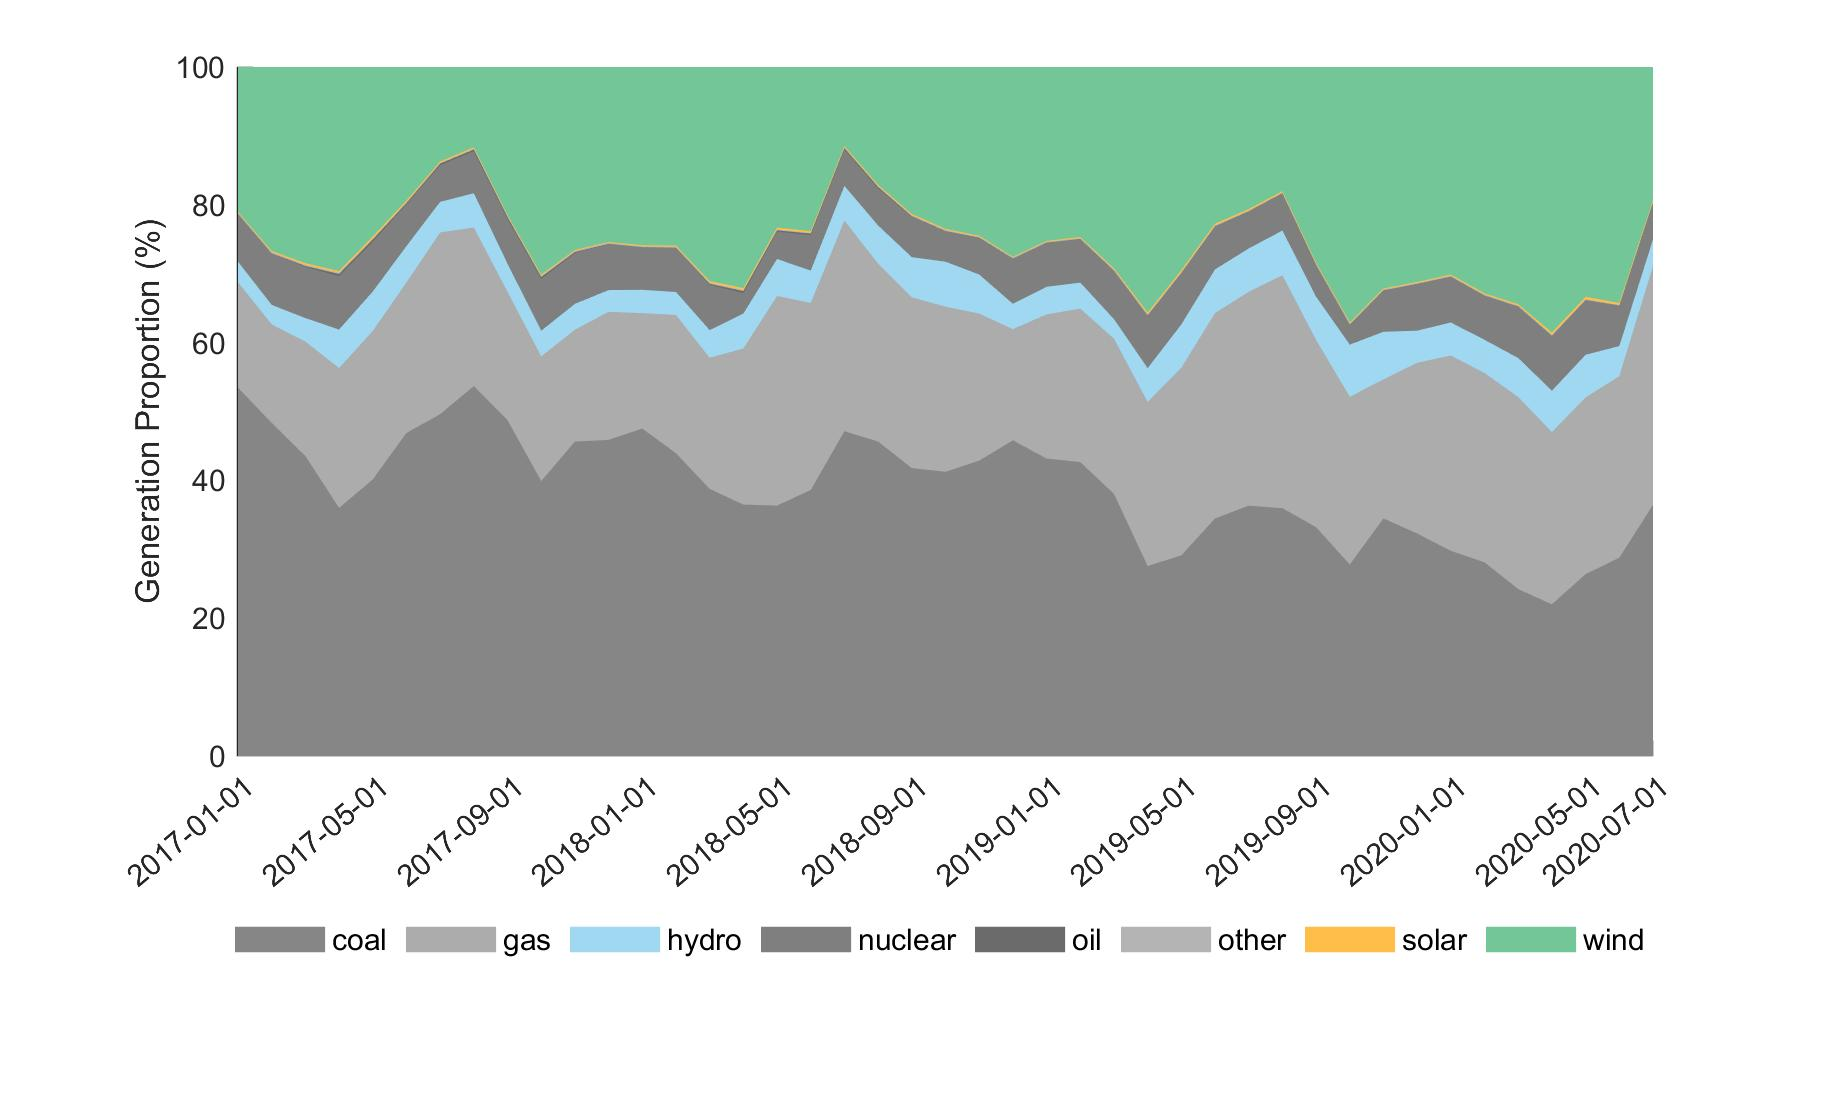
\includegraphics[width=0.8\textwidth]{figures/visualization_example7_2.jpg}
  \caption{Example: Generation Mix of SPP (After Highlighting Renewables)} \label{fig:vis_eg7_2}
\end{figure}

The result is displayed in Figure~\ref{fig:vis_eg7_1} and \ref{fig:vis_eg7_2}, where the color of all fuel types except hydro, solar and wind are changed to gray after the graph is plotted. Therefore, the renewables are visually highlighted.

Such modifications are obtained by changing property values of certain objects using dot notation. For a list of properties, see \verb!Axes Properties!, \verb!Line Properties!, \verb!Area Properties! and \verb!Histogram Properties!. See the help for each function for details.





%--------------------------------
\newpage
\section{Baseline Estimation} \label{sec:baseline}

\subsection{Date and Week Alignment}

\subsection{Ensemble Backcast Estimation}

\subsection{Abnormal Price Index}

\subsection{Excess Change Rate of Renewable}





%---------------------------------
\newpage
\section{Regression Analysis} \label{sec:regression}

\subsection{Regression Methodology}

\subsection{Factor Analysis}






%------------------------------------------------
\newpage
\section{Acknowledgments} \label{sec:thanks}






%------------------------------------------------
\begin{appendices}

\newpage
\section{Glossary} \label{sec:}


\end{appendices}




\newpage
\section*{Reference} \label{sec:ref}
\addcontentsline{toc}{section}{Reference}

\end{document}
